\chapter{曲线积分与曲面积分}
\section{第一型曲线积分}
\precis{曲线,Peano曲线,简单曲线,简单闭曲线,曲线的弧长,弧长参数,第一型曲线积分}
\begin{quiza}
\woe 计算以下第一型曲线积分:
\begin{quizcs}
\item \(\int_Cxyz\dd s,\) 其中\(C\)为空间曲线\(\begin{cases}
x(t)=\cos t,\\y(t)=\sin t,\\z(t)=t
\end{cases}t\in[0,2\pi]\).
\begin{solution}
由参数方程得
\[\int_Cxyz\dd s=\int_{0}^{2\pi}\cos t\cdot\sin t\cdot t\sqrt{\sin^2 t+\cos^2 t+1}\dd t=-\frac{\sqrt{2}\pi}{2}.\qedhere\]
\end{solution}
\item \(\int_Cx^2\dd s\), 其中\(C\)为平面曲线\(x^{2/3}+ y^{2/3}=1.\)
\begin{solution}
置\(x=\cos^3t,y=\sin^3t,t\in[0,2\pi]\), 从而\[\int_Cx^2\dd s=\int_{0}^{2\pi}\cos^6t\sqrt{9\sin^2t\cos^2t}\dd t=3\int_{0}^{2\pi}\cos^6t\left|\sin t\cos t\right|\dd t=\frac{3}{2}.\qedhere\]
\end{solution}
\item \(\int_C|xy|\dd s\), 其中\(C\)为平面曲线\((x^2+y^2)^2=x^2-y^2\).
\begin{solution}
置\(x=\sqrt{\cos 2t}\cos t,y=\sqrt{\cos 2t}\sin t,t\in\left[0,\frac{\pi}{4}\right]\), 利用对称性则有\[\int_C|xy|\dd s=4\int_{0}^{\pi/4}\frac{\cos 2t\cdot\cos t\cdot\sin t}{\sqrt{\cos 2t}}\dd t=\int_{0}^{\pi/2}\sin x\cos^{1/2}x\dd x=\frac{1}{2}B\left(1,\frac{3}{4}\right)=\frac{2}{3}.\qedhere\]
\end{solution}
\end{quizcs}
\end{quiza}
\begin{quizb}
\woe 试将定积分的一些性质移植到第一型曲线积分.
\begin{solution}

\end{solution}
\end{quizb}
\section{第一型曲面积分}
\precis{曲面,同胚,\(k\)维\(C^m\)曲面,Schwarz的例子,集合的面积,分片\(C^m\)曲面,\(\mathbb{R}^n\)中子集的\(k\)维体积(面积),第一型曲面积分,余面积公式,楔积}
\begin{quiza}
\woe 设\(a,b>0\), 计算椭圆柱面\(\frac{x^2}{a^2}+\frac{y^2}{b^2}=1\)在\(z\geqslant 0,y\geqslant 0\)中夹在平面\(y=z\)和平面\(z=0\)之间部分的侧面积.
\begin{solution}
记\(L\)为在\(xOy\)平面上的曲线\(\frac{x^2}{a^2}+\frac{y^2}{b^2}=1\), 结合题设有\(\frac{x^2}{a^2}+\frac{z^2}{b^2}=1\), 即\(z(x)=b\sqrt{1-\frac{x^2}{a^2}}\), 于是面积可以表成以下第一型曲线积分\[\int_Lz(x)\dd s=\int_{0}^{\pi}b\sqrt{1-\cos^2\theta}\sqrt{a^2\cos^2\theta+b^2\sin^2\theta}\dd\theta.\]

\tcbline
选取\(x,z\)为参数, 则由\(\frac{x^2}{a^2}+\frac{y^2}{b^2}=1\)与\(y=z\)得到题设区域到\(xOz\)面的投影\[D=\left\lbrace(x,z)\Big| \frac{x^2}{a^2}+\frac{z^2}{b^2}\leqslant  1,z\geqslant 0 \right\rbrace .\]又记\(F=\frac{x^2}{a^2}+\frac{y^2}{b^2}-1=0\), 则有\(y_x=-\frac{F_x}{F_y}=-\frac{b^2x}{a^2y}\), 于是题设区域的面积\[S=\iint_D\sqrt{1+y_x^2}\dd x\dd z,\]置\(x=ar\cos\theta,z=br\sin\theta\), 结合\(\frac{x^2}{a^2}+\frac{y^2}{b^2}=1\), 代入\(y_x\), 则有\[\begin{split}
S=\iint_D\sqrt{1+y_x^2}\dd x\dd z=\int_{0}^{\pi}\dd\theta\int_{0}^{1}\sqrt{1+\frac{b^2r^2\cos^2\theta}{a^2\left(1-r^2\cos^2\theta\right)}}\cdot abr\dd r
\end{split}\]
\end{solution}
\woe 计算螺旋面\(\begin{cases}
x=r\cos\theta,\\y=r\sin\theta,\\z=a\theta
\end{cases}\left(r\in[0,R],\theta\in[0,2\pi]\right)\)的面积.
\tcbline
记\(\boldsymbol{r}(r,\theta)=\left(r\cos\theta,r\sin\theta,a\theta\right)\), 从而\(\boldsymbol{r}_r=\left(\cos\theta,\sin\theta,0\right),\boldsymbol{r}_{\theta}=\left(-r\sin\theta,r\cos\theta,a\right)\), 于是题设曲面的面积\(\left(D=\left\lbrace(r,\theta)\big|r\in[0,R],\theta\in[0,2\pi]\right\rbrace\right)\)\[\begin{split}
S&=\iint_{D}\left|\boldsymbol{r}_u\times\boldsymbol{r}_{\theta}\right|\dd r\dd\theta=\int_{0}^{2\pi}\dd\theta\int_{0}^{R}\sqrt{a^2+r^2}\,\dd r\\&=\pi R\sqrt{a^2+R^2}+\pi a^2\ln\left(\frac{R+\sqrt{a^2+R^2}}{a}\right).
\end{split}\]
\tcbline 
\woe 设\(\varSigma\)为三角形\(x+y+z=1(x,y,z\geqslant 0)\), 计算第一型曲面积分\(\iint_{\varSigma}\frac{1}{x+2y+3z}\dd S\). 计算曲面积分\(\int_{\varSigma}x^2\dd S\).
\tcbline
\begin{gather*}
\iint_{\varSigma}\frac{1}{x+2y+3z}\dd S=\int_{0}^{1}\dd x\int_{0}^{1-x}\frac{\sqrt{3}\,\dd y}{3-2x-y}=\sqrt{3}\int_{0}^{1}\ln\left(\frac{3-x}{2-x}\right)\dd x=\sqrt{3}\ln\frac{27}{16}.\\
\iint_{\varSigma}x^2\dd S=\int_{0}^{1}\dd x\int_{0}^{1-x}x^2\dd y=\int_{0}^{1}x^2(1-x)\dd x=\frac{1}{12}.
\end{gather*}
\tcbline
\woe 设球面\(x^2+y^2+z^2=R^2\)上均匀分布着单位面积质量为\(\rho\)的物质. 某质点质量为\(m\), 位于点\((0,0,r),r\ne R\). 试求球面上的物质的质量以及球面对于该质点的引力.
\begin{solution}

\end{solution}
\woe 设\(\ell\)是长为\(L\)且足够光滑的平面闭曲线. 对于\(\delta>0\), 设\(W_{\delta}\)为所有以\(\ell\)上的点为球心, \(\delta\)为半径的球的并. 证明: 当\(\delta\)足够小时, \(W_{\delta}\)的表面积为\(2\pi\delta L\).
\tcbline
当\(\delta\)足够小时, \(W_\delta\)暴露在外的面积为\[\int_{0}^{L}\int_{0}^{2\pi}\theta\delta\dd\theta\dd L=2\pi\delta L.\]
\tcbline
\woe 设\(\varphi,\psi\)在\([a,b]\)上连续可导. 证明: 曲线\(\begin{cases}
x=\varphi(t),\\y=\psi(t)
\end{cases}(t\in[a,b])\)绕\(x\)轴旋转一周所得到的旋转面的面积为\(2\pi\int_{a}^{b}|\psi(t)|\sqrt{|\varphi'(t)|^2+|\psi'(t)|^2}\,\dd t\).
\tcbline
曲线绕\(x\)轴旋转一周得到旋转面的面积\(S\)正是\[\begin{split}
\sup\left\lbrace\sum_{j=1}^{N}2\pi \alpha_j\left|E_j\right|\Big|\sum_{j=1}^{N}\alpha_j\chi_{E_j}\text{为}[a,b]\text{上的简单函数, }0\leqslant\sum_{j=1}^{N}\alpha_j\chi_{E_j}\leqslant|y|\right\rbrace,
\end{split}\]记题设曲线为\(L\), 于是\(S=2\pi\int_L|y|\dd s=2\pi\int_{a}^{b}|\psi(t)|\sqrt{|\varphi'(t)|^2+|\psi'(t)|^2}\,\dd t.\)
\end{quiza}

\begin{quizb}
\woe 设\(a,b,c\)为实数, \(A=\sqrt{a^2+b^2+c^2}, f\in L^1[-A,A]\), 证明Poisson(泊松)公式\[\iint\limits_{x^2+y^2+z^2=1}f(ax+by+cz)\dd S=2\pi\int_{-1}^{1}f(Au)\dd u.\]
\begin{proof}
我们对坐标系\(Oxyz\)进行旋转, 记新坐标系为\(Ouvw\), 平面\(Ovw\)即为\(ax+by+cz=0\), \(u\)轴垂直于该平面, 于是有 \[u=\frac{ax+by+cz}{\sqrt{a^2+b^2+z^2}}.\]则有\[\iint\limits_{x^2+y^2+z^2=1}f(ax+by+cz)\dd S=\iint\limits_{u^2+v^2+w^2=1}f(Au)\dd S,\]于是有\(v^2+w^2=\left(\sqrt{1-u^2}\right)^2\), 则令\[u=u,\quad v=\sqrt{1-u^2}\cos\theta,\quad w=\sqrt{1-u^2}\sin\theta,\]
\end{proof}

\end{quizb}
\section{第二型曲线积分}
\precis{第二型曲线积分,第一、二型曲线积分的关系,曲线的方向,Jordan闭曲线定理}

\begin{quiza}
\woe 计算以下第二型曲线积分:
\begin{quizs}
\item \(\int_{C}y\ee^{xy}\cos z\dd x+x\ee^{xy}\cos z\dd y-\ee^{xy}\sin z\dd z,\) 其中\(C\)为曲线\(\begin{cases}
x(t)=\cos t,\\y(t)=\sin t,\\z(t)=t
\end{cases}\)对应于\(t\)从\(0\)到\(2\pi\)的那一段.
\item \(\int_C (3x+2y)\dd x+(x^2-y^2)\dd y\), 其中\(C\)为平面闭曲线\(x^{2/3}+y^{2/3}=1\)的逆时针方向.
\end{quizs}
\begin{solution}
(1)由题意知\[\int_{C}y\ee^{xy}\cos z\dd x+x\ee^{xy}\cos z\dd y-\ee^{xy}\sin z\dd z=\int_{0}^{2\pi}\ee^{\sin t\cos t}\left(\cos 2t-\sin t\right)\dd t,\]首先由
\[\begin{split}
\int_{0}^{2\pi}\ee^{\sin t\cos t}\sin t\dd t&=\int_{0}^{\pi}\ee^{\sin t\cos t}\sin t\dd t+\int_{\pi}^{2 \pi}\ee^{\sin t\cos t}\sin t\dd t\\&=\int_{0}^{\pi}\ee^{\sin t\cos t}\sin t\dd t-\int_{0}^{\pi}\ee^{\sin x\cos x}\sin x\dd x=0,\end{split}\]其次\[\int_{0}^{\pi}\ee^{\sin t\cos t}\cos 2t\dd t=\left.\ee^{\sin t\cos t}\right|^{2\pi}_0=0,\]于是原积分为0.

(2)置\(x=\cos^3t,y=\sin^3t\), \(t\)从\(0\)到\(2\pi\), 于是
\[\begin{split}
&\int_C (3x+2y)\dd x+(x^2-y^2)\dd y\\
=&\int_{0}^{2\pi}\left(3\left(\cos^6t-\sin^6t\right)\sin^2t\cos t-3(3\cos^3t+2\sin^3t)\cos^2t\sin t\right)\dd t\\
=&-6\int_{0}^{2\pi}\sin^4t\cos^2t\dd t=-\frac{3}{4}\pi.\qedhere
\end{split}\]
\end{solution}
\woe 设\(C\)为\(\mathbb{R}^2\)中\(C^1\)简单曲线. \(P,Q\)为\(C\)上的连续函数, 证明\(\left|\int_C P\dd x+Q\dd y\right|\leqslant \int_C\sqrt{P^2+Q^2}\dd s\). 
\begin{proof}

\[
\left|\int_{C}P\dd x+Q\dd y\right|=\left|\int_C\left(P,Q\right)\cdot \dd \boldsymbol{s}\right|=\int_C\left|\left(P\cos\alpha+Q\sin\alpha\right)\dd s\right|\leqslant\int_C\left|P\cos\alpha+Q\sin\alpha\right|\dd s,\]由Cauchy不等式知\(\left|P\cos\alpha+Q\sin\alpha\right|\leqslant\sqrt{P^2+Q^2}\cdot\sqrt{\cos^2\alpha+\sin^2\alpha}\), 命题获证.
\end{proof}
\end{quiza}
\begin{quizb}
\woe 对于\(\mathbb{C}\)中的\(C^1\)曲线\(C\)及其上的复值连续函数\(f\), 记\(f(z)\dd z=f(x+\mathrm{i}y)(\dd x+\mathrm{i}\dd y)=f(x+\mathrm{i}y)\dd x+\mathrm{i}f(x+\mathrm{i}y)\dd y\). 若令\(s\)为\(C\)的弧长参数, \(C_{s,\Delta s}\)为\(C\)上对应于弧长从\(s\)到\(s+\Delta s\)的那一段, 则\(\lim_{\Delta s\rightarrow 0}\frac{\left|\int_{C_s,\Delta s}\dd z\right|}{|\Delta s|}=1.\)这样相当于\(|\dd z|=\dd s\). 证明: \(\left|\int_C f(z)\dd z\right|\leqslant \int_C|f(z)|\dd s\). 
\begin{proof}
利用题设条件与Cauchy不等式有:\[\begin{split}
&\left|\int_Cf(z)\dd z\right|=\left|\int_C f(x+\mathrm{i}y)\dd x+\mathrm{i}f(x+\mathrm{i}y)\dd y\right|\\
\leqslant&\int_C\left|\left(f(x+\mathrm{i}y),\mathrm{i}f(x+\mathrm{i}y)\right)\cdot (\dd x,\dd y)\right|\leqslant\int_C|f(z)|\dd s \qedhere
\end{split}\]
\end{proof}
\end{quizb}

\section{第二型曲面积分}
\precis{第二型曲面积分,第一、二型曲面积分的关系,通量,曲面的侧}
\begin{quiza}
\woe 计算以下第二型曲面积分:
\begin{quizs}
\item  \(\iint_{\varSigma}(x+y)\dd y\dd z+(y+z)\dd z\dd x+(z+x)\dd x\dd y\), 其中\(\varSigma\)为曲面\(x^2+\frac{y^2}{4}+\frac{z^2}{9}=1\)的上半部分, 方向取上侧.
\item \(\iint_{\varSigma}x^2\dd y\dd z+y^2\dd z\dd x+(z+2)^2\dd x\dd y\), 其中\(\varSigma\)为锥面\(z=\sqrt{x^2+y^2}\)对应于\(0\leqslant z\leqslant 1\)的那部分, 方向取上侧.
\end{quizs}
\begin{solution}
(1)为计算\(\iint_{\varSigma}(x+y)\dd y\dd z\), 将\(\varSigma\)投影到\(yz\)平面, 其投影为\[D_1=\left\lbrace(y,z)\big|\frac{y^2}{4}+\frac{z^2}{9}\leqslant 1,z\geqslant 0\right\rbrace.\]曲面分为两部分:\[\begin{split}
\varSigma_1&=\left\lbrace (x,y,z)\big|x=\sqrt{1-\frac{y^2}{4}-\frac{z^2}{9}},(y,z)\in D_1 \right\rbrace,\text{方向为前侧},\\
\varSigma_2&=\left\lbrace (x,y,z)\big|x=-\sqrt{1-\frac{y^2}{4}-\frac{z^2}{9}},(y,z)\in D_1 \right\rbrace,\text{方向为后侧}.
\end{split}\]于是\[\begin{split}
\iint_{\varSigma}(x+y)\dd y\dd z&=\iint_{\varSigma_1}(x+y)\dd y\dd z+\iint_{\varSigma_2}(x+y)\dd y\dd z\\
&=\iint_{D_1}\left(\sqrt{1-\frac{y^2}{4}-\frac{z^2}{9}}+y\right)\dd y\dd z+\iint_{D_1}\left(\sqrt{1-\frac{y^2}{4}-\frac{z^2}{9}}-y\right)\dd y\dd z\\&=2\iint_{D_1}\sqrt{1-\frac{y^2}{4}-\frac{z^2}{9}}\dd y\dd z=4\pi.
\end{split}\]
同理计算可得\(\iint_{\varSigma}(y+z)\dd z\dd x=4\pi,\,\iint_{\varSigma}(z+x)\dd x\dd y=4\pi\). 从而\[\iint_{\varSigma}(x+y)\dd y\dd z+(y+z)\dd z\dd x+(z+x)\dd x\dd y=12\pi.\]

(2)由对称性\[\iint_{\varSigma}x^2\dd y\dd z=\iint_{\varSigma}y^2\dd z\dd x=0.\]于是仅需计算\[\iint_{\varSigma}(z+2)^2\dd x\dd y=\iint\limits_{x^2+y^2\leqslant 1}\left(\sqrt{x^2+y^2}+2\right)^2\dd x\dd y=\frac{43}{6}\pi.\]
\end{solution}
\woe 设\(\varSigma\)为\(\mathbb{R}^3\)中的有向\(C^1\)曲面, \(P,Q,R\)为\(\varSigma\)上的连续函数. 证明:\[\left|\iint_{\varSigma}P\dd y\dd z+Q\dd z\dd x+R\dd x\dd y\right|\leqslant\iint_{\varSigma}\sqrt{P^2+Q^2+R^2}\dd S.\]
\begin{proof}
由第一, 第二型曲面积分的关系与Cauchy不等式得到\[\left|\iint_{\varSigma}P\dd y\dd z+Q\dd z\dd x+R\dd x\dd y\right|=\left|\iint_{\varSigma}\left(P,Q,R\right)\cdot\boldsymbol{n}(\boldsymbol{x})\dd S\right|\leqslant\iint_{\varSigma}\sqrt{P^2+Q^2+R^2}\dd S.\]其中\(\boldsymbol{n}\)为\(\varSigma\)对应的单位法向量.
\end{proof}
\end{quiza}
\begin{quizb}
\woe 若请你对\(\mathbb{R}^3\)中的曲面\(\varSigma\)即函数\(P\)定义\(\iint_{\varSigma}P(x,y,z)\dd y\dd z\), 则对于\(\varSigma\)和\(P\)的要求要怎么提? 
\begin{solution}

\end{solution}
\end{quizb}
\section{Green公式,Gauss公式,Stokes公式}
\precis{向量场,单连通域,Ostrogradsky-Gauss定理(散度定理),Green公式,Stokes公式,曲线积分和路径无关性,原函数的存在性,循环常数,场论初步,梯度场(保守场),散度场,向量线,环量,旋度,无源场,无旋场,Hamilton算子,Laplace算子,分部积分公式,Green第一、第二公式}
\begin{quiza}
\woe 计算以下曲线积分绕原点的循环常数:\vspace{8pt}\\\vspace{8pt}
\begin{tabular}{lcccl}
\((1)\int_C\frac{-y\dd x+x\dd y}{x^2+y^2}\)&&&\((2)\int_{C}\frac{x\dd x+y\dd y}{x^2+y^2}\).
\end{tabular}
\begin{solution}
不妨取\(C=\{(x,y)\big|x^2+y^2=1\}\), 置\(x=\cos\theta,y=\sin\theta,(\theta\in[0,2\pi])\), 于是得到\[\int_C\frac{-y\dd x+x\dd y}{x^2+y^2}=2\pi,\quad\int_{C}\frac{x\dd x+y\dd y}{x^2+y^2}=0.\qedhere\]
\end{solution}
\woe 设曲线\(C\)为\(\begin{cases}
x=\cos t,\\y=2t\sin t,\\z=t
\end{cases}\)对应于\(t\)从\(0\)到\(2\pi\)的第一段. 试计算\[\int_C\ee^{xy}\left[\left(y\cos(x+y)+yz^2-\sin(x+y)\right)\dd x+\left(x\cos(x+y)+xz^2-\sin(x+y)\right)\dd y+2z\dd z \right].\]
\begin{solution}
方便起见设原积分为\(\int_CP\dd x+Q\dd y+R\dd z\). 令\(L\)为直线段\(x=1,y=0,z\)从\(2\pi\)跑到\(0\), 于是\(C\cup L\)为闭曲线, 任取曲面\(\varSigma\)以\(C\cup L\)为边界, 方向与\(C\cup L\)的方向成右手系, 由Stokes公式得到\[\int_{C\cup L}P\dd x+Q\dd y+R\dd z=\iint_{\varSigma}\left(\frac{\partial R}{\partial y}-\frac{\partial Q}{\partial z}\right)\dd y\dd z+\left(\frac{\partial P}{\partial z}-\frac{\partial R}{\partial x}\right)\dd z\dd x+\left(\frac{\partial Q}{\partial x}-\frac{\partial P}{\partial y}\right)\dd x\dd y=0.\]从而\[\int_CP\dd x+Q\dd y+R\dd z=-\int_LP\dd x+Q\dd y+R\dd z=\int_{0}^{2\pi}2\ee z\dd z=4\ee\pi^2.\qedhere\]
\end{solution}
\woe 设\(R>0\), 计算积分\(\iint_{\varSigma}\frac{Rx\,\dd y\dd z+(z+R)^2\,\dd x\dd y}{\sqrt{x^2+y^2+z^2}}\), 其中\(\varSigma\)为下半球面\(z=-\sqrt{R^2-x^2-y^2}\)的上侧.
\begin{solution}
记原积分为\(I_2\), 选取平面\(D=\{(x,y,z)\big|x^2+y^2\leqslant R^2,z=0\}\), 方向为上侧, 可以得到\[I_2:=\iint_{D}\frac{Rx\dd y\dd z+(z+R)^2\dd x\dd y}{\sqrt{x^2+y^2+z^2}}=\iint_{D}\frac{R^2}{\sqrt{x^2+y^2}}\dd x\dd y=2\pi R^3.\]记\(\varOmega\)为\(\varSigma\cup D\)的内部, 于是由Gauss公式\[\begin{split}
-I_1+I_2&=\iiint_{\varOmega}\left(\frac{\partial}{\partial x}\left(\frac{Rx}{\sqrt{x^2+y^2+z^2}}\right)+\frac{\partial}{\partial z}\left(\frac{(z+R)^2}{\sqrt{x^2+y^2+z^2}}\right)\right)\dd x\dd y\dd z\\
=&\frac{13}{6}\pi R^3+\pi R^2-\frac{2}{3}\pi^2R^3
\end{split}\]于是\(I_1=\frac{2}{3}\pi^2R^3-\pi R^2-\frac{1}{6}\pi R^3.\)
\end{solution}
\woe 设\(S\)为椭球面\(\frac{x^2}{2}+\frac{y^2}{2}+z^2=1\)的上半部分\((z>0)\), 对于\(P=(x,y,z)\in S\), \(\varSigma\)为\(S\)在点\(P\)处的切平面, \(\rho(x,y,z)\)为原点到平面\(\varSigma\)的距离, 求积分\(\iint_{S}\frac{z}{\rho(x,y,z)}\dd S\).
\begin{solution}
首先, 记\(f=\frac{x^2}{2}+\frac{y^2}{2}+z^2-1\), 对于\(P=(A,B,C)\in S\), \(\varSigma\)的方程为\[\left(f_x\big|_{x=A},f_y\big|_{y=B},f_z\big|_ {z=C}\right)\cdot (x-A,y-B,z-C)=0,\]即\(Ax+By+2Cz-A^2-B^2-2C^2=0.\)由此\[\rho(x,y,z)=\frac{x^2+y^2+2z^2}{\sqrt{x^2+y^2+4z^2}},\]即计算\(\iint_{S}\frac{z\sqrt{x^2+y^2+4z^2}}{x^2+y^2+2z^2}\dd S.\) 注意到\(\varSigma\)上的点\((x,y,z)\)处, 指向曲面外侧的的单位法向量为\(\frac{(x,y,2z)}{\sqrt{x^2+y^2+4z^2}}\), 这样就是计算\[I(S):=\iint_{S}\frac{zx}{x^2+y^2+2z^2}\,\dd y\dd z+\frac{zy}{x^2+y^2+2z^2}\,\dd z\dd x+\frac{2z^2}{x^2+y^2+2z^2}\,\dd x\dd y.\]置\(D=\{(x,y,z)\big| \frac{x^2}{2}+\frac{y^2}{2}=1,z=0\}\), 易见\(I(D)=0\). 令\(\varOmega\)表示\(S\cup D\)的内部, 利用Gauss公式, 得到\[\begin{split}
I&=\iiint_{\varOmega}\frac{6z(x^2+y^2+2z^2)-2x^2z-2y^2z-8z^3}{(x^2+y^2+2z^2)^2}\dd x\dd y\dd z\\&=\int_{0}^{2\pi}\dd\theta\int_{0}^{\pi/2}\dd\varphi\int_{0}^{1}\left(6r\cos\varphi\sin\varphi-2r\cos\varphi\sin^3\varphi-4r\cos^3\varphi\sin\varphi\right)\dd r=\frac{\pi}{2}.\qedhere
\end{split}\]
\end{solution}
\woe 设\(\theta_1<\theta_2\leqslant\theta_1+2\pi\). 证明: 在极坐标下由射线\(\theta=\theta_1,\theta=\theta_2\)和曲线\(C:\rho=\rho(\theta)(\theta_1\leqslant \theta\leqslant\theta_2)\)所围成的曲边扇形(如图\ref{fig:m}所示)的面积为\(\frac{1}{2}\int_{\theta_1}^{\theta_2}\rho^2\left(\theta\right)\dd\theta\). 当\(\rho\)连续可导时, 验证这一结果与公式(11.5.9)给出的结果一致. 思考这一面积为什么不是\(\frac{1}{2}\int_C\rho^2\dd\sigma\).
\begin{figure}[H]
\centering
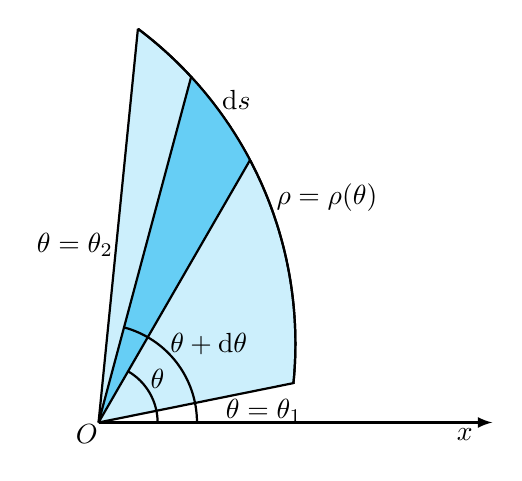
\begin{tikzpicture}[scale=0.5]
\begin{scope}
 \clip (1,10) rectangle (5.1,1);
  \filldraw[fill=cyan!20,draw=black,thick] (-5,2) circle [radius=10];
   \fill[color=cyan!60!white](60:7.7)--(75:9.1)--(70:8.6);
   \fill[color=cyan!60!white](60:7.7)--(75:9.1)--(65:8.16);
   \fill[color=cyan!60!white](60:7.7)--(75:9.1)--(0,0);
   \draw[black,thick] (-5,2) circle [radius=10];
\end{scope}
\begin{scope}
\fill[color=cyan!20](0,0)--(1,10)--(1,3)--(4.9498,1);
\draw[-latex,thick] (0,0)--(10,0);
\draw[thick](0,0)--(1,10);`
\draw[thick](0,0)--(4.9498,1);`
\end{scope}
\begin{scope}
\fill[color=cyan!60!white](60:7.5)--(75:9)--(0,0);
\draw[thick] (75:9.1)--(0,0);
\draw[thick] (60:7.7)--(0,0);
\end{scope}
\draw[thick] (1.5,0) arc (0:60:1.5);
\draw[thick] (2.5,0) arc (0:75:2.5);
\node at (1.5,1.1) {$\theta$};
\node at (4.2,0.3) {$\theta=\theta_1$};
\node at (2.8,2) {$\theta+\mathrm{d}\theta$};
\node at (-0.6,4.5) {$\theta=\theta_2$};
\node at (3.5,8.2) {$\mathrm{d}s$};
\node at (5.8,5.7) {$\rho=\rho(\theta)$};
\node at (-0.3,-0.3) {$O$};
\node at (9.3,-0.3) {$x$};
\end{tikzpicture}
\caption{第5题图}
\label{fig:m}
\end{figure}
\begin{solution}
\end{solution}
\woe 试对于足够光滑的\(f\)和\(\boldsymbol{F}\), 化简以下表达式:\\
\begin{tabular}{lclclclcl}
\((1)\nabla\cdot\nabla f\);&&\((2)\nabla\times\nabla f\);&&\((3)\nabla\left(\nabla\cdot\boldsymbol{F}\right)\);&&\((4)\nabla\cdot\left(\nabla\times\boldsymbol{F}\right)\);&&\((5)\nabla\times\left(\nabla\times\boldsymbol{F}\right)\).
\end{tabular}
\begin{solution}
不妨设\(f=f(x,y,z),\boldsymbol{F}=X(x,y,z)\boldsymbol{i}+Y(x,y,z)\boldsymbol{j}+Z(x,y,z)\boldsymbol{z}\), 于是\[\nabla\cdot\nabla f=\nabla\cdot\left(\frac{\partial f}{\partial x}\boldsymbol{i}+\frac{\partial f}{\partial y}\boldsymbol{j}+\frac{\partial f}{\partial z}\boldsymbol{k}\right)=\frac{\partial^2f}{\partial x^2}+\frac{\partial^2f}{\partial y^2}+\frac{\partial^2f}{\partial z^2}.\]容易验证\(\nabla\times\nabla f=\boldsymbol{0},\nabla\cdot\left(\nabla\times\boldsymbol{F}\right)=0\).
\[\nabla\left(\nabla\cdot\boldsymbol{F}\right)=\left(\frac{\partial}{\partial x}\left(\frac{\partial X}{\partial x}+\frac{\partial Y}{\partial y}+\frac{\partial Z}{\partial z}\right),\frac{\partial}{\partial x}\left(\frac{\partial X}{\partial x}+\frac{\partial Y}{\partial y}+\frac{\partial Z}{\partial z}\right),\frac{\partial}{\partial z}\left(\frac{\partial X}{\partial x}+\frac{\partial Y}{\partial y}+\frac{\partial Z}{\partial z}\right)\right),\]
\[\begin{split}
&\nabla\times\left(\nabla\times\boldsymbol{F}\right)=\nabla\times\left(\frac{\partial Z}{\partial y}-\frac{\partial Y}{\partial z},\frac{\partial X}{\partial z}-\frac{\partial Z}{\partial x},\frac{\partial Y}{\partial x}-\frac{\partial X}{\partial y}\right)\\=&\left(\frac{\partial^2Y}{\partial x\partial y}-\frac{\partial^2X}{\partial y^2}-\frac{\partial^2X}{\partial z^2}+\frac{\partial^2Z}{\partial x\partial z},\frac{\partial^2Z}{\partial y\partial z}-\frac{\partial^2Y}{\partial z^2}-\frac{\partial^2Y}{\partial x^2}+\frac{\partial^2X}{\partial y\partial x},\frac{\partial^2X}{\partial z\partial x}-\frac{\partial^2Z}{\partial x^2}-\frac{\partial^2Z}{\partial y^2}+\frac{\partial^2Y}{\partial z\partial y}\right).
\end{split}\]值得一提的是\(\nabla\left(\nabla\cdot\boldsymbol{F}\right)-\nabla\times\left(\nabla\times\boldsymbol{F}\right)=\Delta\boldsymbol{F}\).
\end{solution}
\woe 保守场, 无源场和无旋场之间有没有什么关系?
\begin{solution}
content...
\end{solution}
\woe 用记号\(\nabla\)重写Gauss公式和Stokes公式.
\begin{solution}
Gauss公式可以表示为\[\iint_{\partial \varOmega}\boldsymbol{F}\cdot\dd\boldsymbol{S}=\iiint_{\varOmega}\nabla\cdot\boldsymbol{F}\dd V,\]Stokes公式可表示为\[\int_{\partial\varSigma}\boldsymbol{F}\cdot\dd\boldsymbol{s}=\iint_{\varSigma}\left(\nabla\cdot\boldsymbol{F}\right)\cdot\dd\boldsymbol{S}.\qedhere\]
\end{solution}
\woe 验证\[\int_{\partial\varOmega}\omega=\int_{\varOmega}\mathrm{d}\omega\]适用于Green公式, Ostrogradski\v{\i}-Gauss公式, Stokes公式以及Newton-Leibniz公式.
\begin{solution}

\end{solution}
\woe 试利用Stokes公式计算\(\int_Cy\dd x+2z\dd y+3x\dd z\), 其中\(C\)为圆周\(\begin{cases}
x^2+y^2+z^2=1,\\x+y+z=0.
\end{cases}\)从\(z\)轴正向\footnote{表示从上往下看.}看去, 曲线是逆时针方向的.
\begin{solution}
平面\(x+y+z=0\)的法线的方向余弦为\(\cos\alpha=\cos\beta=\cos\beta=\frac{1}{\sqrt{3}}\), 于是由Stokes公式\[\int_Cy\dd x+2z\dd y+3x\dd z\]
\end{solution}
\end{quiza}
\begin{quizb}
\woe 设\(a,b,c>0,\) \(\varSigma\)为曲面\(\frac{x^2}{a^2}+\frac{y^2}{b^2}+\frac{z^2}{c^2}=1.\) 利用Gauss公式计算曲面积分\[\iint_{\varSigma}\frac{\dd S}{(x^2+y^2+z^2)^{3/2}\sqrt{\displaystyle\frac{x^2}{a^4}+\frac{y^2}{b^4}+\frac{z^2}{c^4}}}.\]
\begin{solution}
记原积分为\(I\), 注意到有\[I=\iint_{\varSigma}\frac{\displaystyle\frac{x^2}{a^2}+\frac{y^2}{b^2}+\frac{z^2}{y^2}}{(x^2+y^2+z^2)^{3/2}\sqrt{\displaystyle\frac{x^2}{a^4}+\frac{y^2}{b^4}+\frac{z^2}{c^4}}}\dd S.\]
注意到曲面\(\varSigma\)的单位法向量为\(\frac{\left(x/a^2,y/b^2,z/c^2\right)}{\sqrt{x^2/a^4+y^2/b^4+z^2/c^4}}\). 于是有\[I=\iint_{\varSigma}\frac{x\dd y\dd z+y\dd z\dd x+z\dd x\dd y}{\left(x^2+y^2+z^2\right)^{3/2}}=:\iint_{\varSigma}P \dd z+Q\dd z\dd x+R\dd x\dd y,\]由于\(P,Q,R\)在原点处不可导, 而在别处有\[\frac{\partial P}{\partial x}+\frac{\partial Q}{\partial y}+\frac{\partial R}{\partial z}=0,\]再由Gauss公式有\[I=\iint_{\varSigma'}\frac{\dd S}{x^2+y^2+z^2}=\iint_{\varSigma'}\frac{\dd S}{\rho^2}=\frac{4\pi\rho^2}{\rho^2}=4\pi,\]其中\(\varSigma'\)是半径\(\rho\)充分小使得含于\(\varSigma\)的球面\(x^2+y^2+z^2=\rho^2\).
\end{solution}
\woe 设\(\boldsymbol{A}\)是\(n\)阶方阵, \(\varOmega\)为\(\mathbb{R}^n\)中具有\(C^1\)边界的有界区域, \(\boldsymbol{\varphi}\in C^2_0(\varOmega;\mathbb{R}^n)\). 证明: \[\int_{\varOmega}\mathrm{det}\left(\boldsymbol{A}+\boldsymbol{\varphi_x}\right)\dd x=\mathrm{det}(\boldsymbol{A})\left|\varOmega\right|.\]
\begin{proof}

\end{proof}
\woe 设\(n\geqslant 1\), \(R\)是仅在点\(0,0\)为零的\(2n\)次二元多项式, \(P,Q\)是不超过\(2n-2\)次的二元多项式. 若\(\varliminf_{(x,y)\rightarrow\infty}\frac{R(x,y)}{(x^2+y^2)^n}>0\), 且在点\((0,0)\)之外成立\(\frac{\partial}{\partial x}\frac{Q(x,y)}{R(x,y)}=\frac{\partial}{\partial y}\frac{P(x,y)}{R(x,y)}\), 证明: 曲线积分\(\int_{C}\frac{P\dd x+Q\dd y}{R}\)绕点\((0,0)\)的循环常数为零.
\begin{proof}

\end{proof}
\woe 在上一题中, 去掉条件\(\varliminf_{(x,y)\rightarrow\infty}\frac{R(x,y)}{(x^2+y^2)^n}>0\)后结论是否依然成立.
\begin{solution}

\end{solution}
\end{quizb}
\section{调和函数与解析函数}
\precis{调和函数,平均值公式,最值原理,Poisson公式,复可导与复解析的等价性,Cauchy定理,最大模原理,Liouville定理,共轭函数,利用解析函数计算}
\begin{quiza}
\woe 利用解析函数的性质证明: \(\int_{0}^{+\infty}\frac{\ee^{-x}-\cos x}{x}\dd x\).
\begin{proof}

\end{proof}
\woe 设\(1\leqslant p<+\infty\), \(\varphi\)为\(\mathbb{R}^n\)上的调和函数, \(\varphi\in L^p(\mathbb{R}^n)\). 证明\(\varphi\equiv 0\).
\begin{proof}

\end{proof}
\woe 设\(\varphi\in C^2(\mathbb{R}^n)\)为\textit{上调和函数}, 即满足\(-\Delta\varphi\geqslant 0\). 任取\(\boldsymbol{x}_0\in\mathbb{R}^n\), 证明\(F(r)=\frac{1}{|B_r(\boldsymbol{x}_0)|}\cdot\int_{B_r(\boldsymbol{x}_0)}\varphi(\boldsymbol{x})\dd x\)关于\(r>0\)单调.
\begin{proof}

\end{proof}
\woe 设\(f\)在有界复区域\(D\)上复解析, 在\(\overline{D}\)上连续. 若存在\(z_0\in D\)满足\(|f(z_0)|\leqslant\min_{z\in\partial D}|f(z)|\). 证明: \(f\)在\(D\)内为常数或有零点.
\begin{proof}
假设\(f\)不为常数且无零点, 则\(\frac{1}{f(z)}\)在\(D\)上解析, 依条件有\(\left|\frac{1}{f(z_0)}\right|\geqslant\max_{x\in\partial D}\left|\frac{1}{f(z)}\right|\), 这与最大模原理矛盾, 从而\(f\)在\(D\)内有零点.
\end{proof}
\woe 设\(f\)在\(\mathbb{C}\)上复解析, \(\lim_{z\rightarrow\infty}|f(z)|=+\infty\). 证明: \(f\)有零点. 进一步, 若存在\(n\geqslant 1\)使得\(\lim_{z\rightarrow\infty}\frac{|f(z)|}{|z|^n}=a\in\left(0,+\infty\right]\), 则\(f\)至少有\(n\)个零点(含重数).
\begin{proof}
由条件知\(\lim_{z\rightarrow\infty}\left|\frac{1}{f(z)}\right|=0\), 若\(f\)无零点, 则\(\frac{1}{f(z)}\)解析, 但依极限知\(\exists z_0\), 使得\(\forall |z|>|z_0|\)时有\(\left|1/f(z)\right|>\left|1/f(z_0)\right|\), 与最大模原理矛盾, 从而\(f\)有零点. 进一步, 若\(\lim_{z\rightarrow\infty}\frac{\left|f(z)\right|}{|z|^n}=a\in\left(0,+\infty\right]\), 则\(\lim_{z\rightarrow\infty}\left|\frac{f(z)}{z^{n-1}}\right|=+\infty\), 归纳即得结论. 
\end{proof}
\woe 证明: 对任何\(z\in\mathbb{C}\)以及\(\delta\in(0,1)\), 有\(\lim_{s\rightarrow+\infty}\frac{\displaystyle\int_{(0,1-\delta)\cup(1+\delta,+\infty)}x^z\left(x\ee^{-x}\right)^s\dd x}{\displaystyle\int_{0}^{+\infty}\left(x\ee^{-x}\right)^s\dd x}=0.\)
\begin{proof}
记\(\alpha\)为\(x\ee^{-x}\)在\([0,1-\delta]\cup[1+\delta,+\infty]\)上的最大值, 给定\(\beta\in(\alpha,\ee^{-1})\), 则存在长度为\(l\)的区间\(I\subseteq[1-\delta,1+\delta]\), 使得\(x\ee^{-x}\geqslant \beta\)对\(x\in I\)恒成立. 从而\(\int_{0}^{+\infty}\left(x\ee\right)^s\dd x\geqslant l\cdot\beta^s\), \(s\)足够大时, 存在常数\(C_1\)使得\[\left|\int_{0}^{1-\delta}x^z(x\ee^{-x})^{s}\dd x\right|\leqslant C_1\cdot\alpha^s,\]又存在常数\(C_2\)使得\[\begin{split}
&\left|\int_{1+\delta}^{+\infty}x^z(x\ee^{-x})^s\dd x\right|\leqslant\int_{1+\delta}^{+\infty}x^{\mathrm{Re}\,z}(x\ee^{-x})^s\dd x\\&\leqslant\int_{1+\delta}^{+\infty}x^{\mathrm{Re}\, z}(x\ee^{-x})^{s-1}\cdot\left[s(x-1)-\mathrm{Re}\,z\right]\ee^{-x}\dd x=-\int_{1+\delta}^{+\infty}\dd\left[x^{\mathrm{Re}\, z}(x\ee^{-x})^s\right]\leqslant C_2\cdot\alpha^s.\qedhere
\end{split}\]
\end{proof}
\end{quiza}
\begin{quizb}
\woe 设\(\alpha\in\mathbb{R}\), \(\boldsymbol{\sigma}\in S^{n-1}\). 证明: 在\(\mathbb{R}^n\)的单位球\(B_1(\boldsymbol{x})\)内, \(f(\boldsymbol{x})=|\boldsymbol{\sigma}-\boldsymbol{x}|^\alpha\)可以展开成\(\boldsymbol{x}\)的幂级数, 且对任何\(\delta\in(0,1)\), 该幂级数关于\((\boldsymbol{\sigma},\boldsymbol{x})\in S^{n-1}\times B_{\delta}(\boldsymbol{0})\)一致收敛.
\woe 已知当\(0<\alpha<1\)时, 成立\[\sum_{n=1}^{\infty}\frac{1}{n^2-\alpha^2}=\frac{1}{2\alpha^2}-\frac{\pi\cot (\alpha\pi)}{2\alpha}.\]试利用复解析函数的性质证明: 当\(\alpha>0\)时, 成立\[\sum_{n=1}^{\infty}\frac{1}{n^2+\alpha^2}=-\frac{1}{2\alpha^2}+\frac{\pi}{2\alpha\tanh(\alpha\pi)}.\]
\woe 试用不同的方法证明\[\mathrm{sh}\, x=x\prod_{n=1}^{\infty}\left(1+\frac{x^2}{n^2\pi^2}\right).\]
\end{quizb}
\section{附录: \texorpdfstring{\(C^1\)}{}曲面上的Hausdoff测度}
\precis{Binet-Cauchy公式,\(C^1\)曲面的Hausdorff公式}
\begin{theorem}{}{kwei}
设\(1\leqslant k\leqslant n,\) \(D_0\)为\(\mathbb{R}^k\)中得区域, 单射\(\boldsymbol{\varphi}:D_0\rightarrow\mathbb{R}^n\)连续可微, 则对于紧包含于\(D_0\)得可测集\(D,\,\varSigma=\boldsymbol{\varphi}(D)\)得\(k\)维测度为\[V_k(\varSigma)=\int_D\sqrt{\mathrm{det}\left(\boldsymbol{\varphi_u}^T\boldsymbol{\varphi_u}\right)}\dd\boldsymbol{u}.\]等价地,\[V_k(\varSigma)=\int_D\sqrt{\boldsymbol{\varphi_u}\text{的所有}k\text{阶子式的平方和}}\,\dd\boldsymbol{u}.\]
\end{theorem}

\begin{quiza}
\woe 设\(\Omega\subseteq\mathbb{R}^n\)为区域, \(\boldsymbol{\varphi}\in C^1\left(\varOmega;\mathbb{R}^m\right)\). 设\(F\subset \Omega\)为紧集,\[\omega(r)=\underset{0<|\boldsymbol{u}-\boldsymbol{v}|\leqslant r\atop\boldsymbol{u}\in F,\boldsymbol{v}\in\Omega}{\mathrm{sup}}\frac{\left|\boldsymbol{\varphi}(\boldsymbol{u})-\boldsymbol{\varphi}(\boldsymbol{v})\right|}{|\boldsymbol{u}-\boldsymbol{v}|},\quad r>0.\]证明\(\lim_{r\rightarrow 0^+}\omega(r)=0.\)
\begin{proof}

\end{proof}
\end{quiza}
\begin{quizb}
\woe 试减弱定理\reff{Th:kwei} 得条件使得结论仍然成立.
\begin{solution}

\end{solution}
\end{quizb}